\documentclass{beamer}
\usepackage{animate}
\usepackage{multimedia}
\usepackage[english,russian]{babel}

\usepackage{pgfpages}
\setbeameroption{show notes on second screen}
%https://tug.ctan.org/macros/latex/contrib/beamer/doc/beameruserguide.pdf

\usepackage[T2A]{fontenc}
\usepackage[utf8]{inputenc}

\setbeamertemplate{caption}[numbered]

\usetheme{CambridgeUS}
\usecolortheme{dolphin}


\title[Фракталы]{Фракталы}
\author[Быковских Д.А.]{Быковских Дмитрий Александрович}
\date{23.09.2023}

\if 0

\fi

\begin{document}
\begin{frame}
	\titlepage
\end{frame}
%\section{Обзор}
\begin{frame}{Содержание}
		\begin{itemize}
			\item Введение
			% \item История фракталов
			\item Геометрические фракталы
			\item Алгебраические фракталы
			\item Стохастические фракталы
		\end{itemize}
	\end{frame}

	\begin{frame}{Введение}

		\begin{figure}
					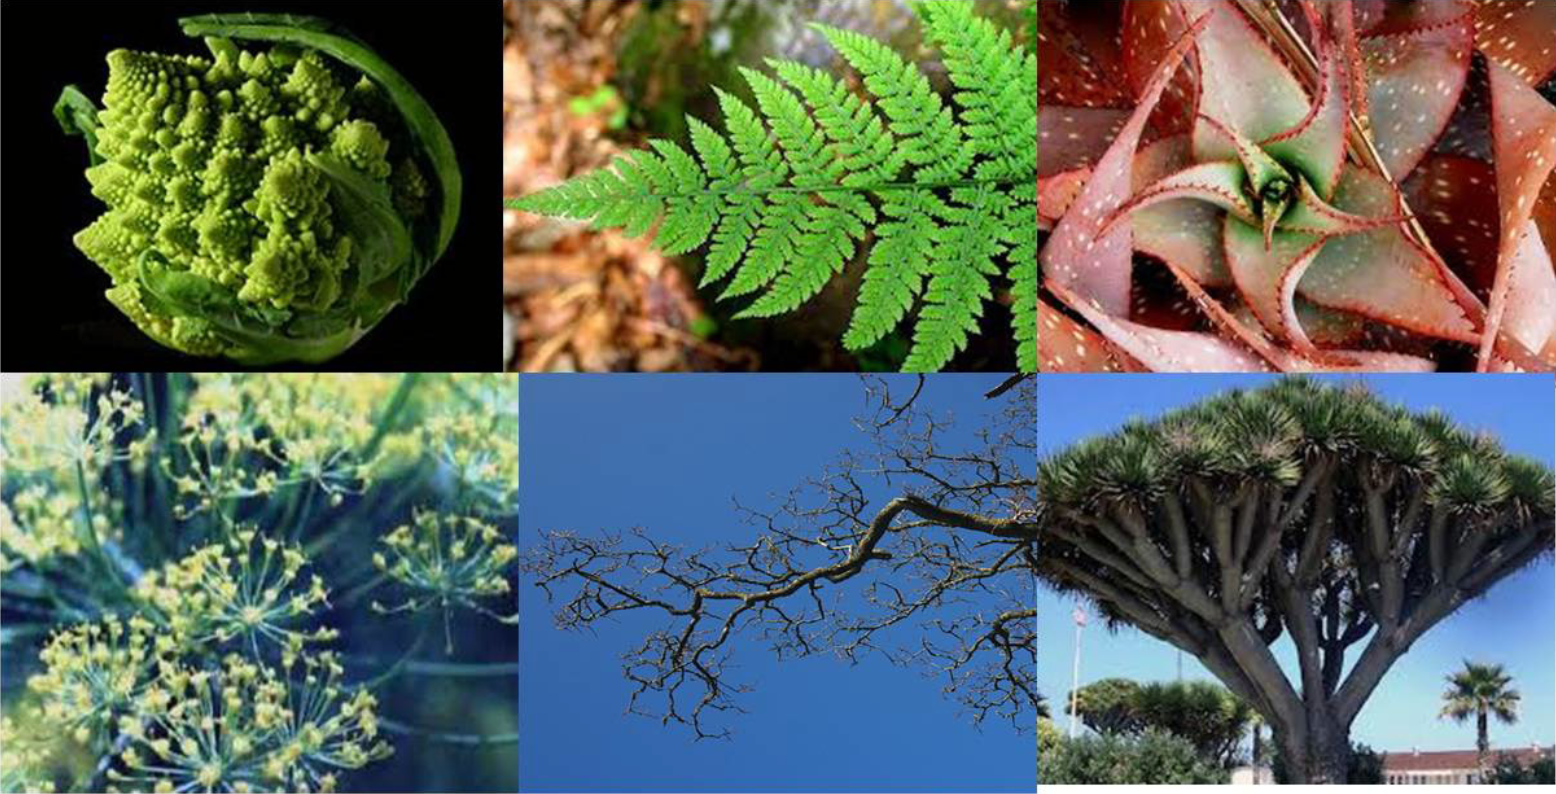
\includegraphics[width=0.9\textwidth]{images/Природа.png}
					\caption{Объекты живой природы}
		\end{figure}
	
		\note{
			Воображение иссякает прежде природы.

			Блез Паскаль
			
			Многие формы природных объектов неправильны и фрагментированы. 
			
			Например, облака, горы, деревья и многое др.
	
			Исследование этих объектов и неспособность их описать с помощью простых геометрических объектов 
			привело к появлению фракталов.

			% Примеры фракталов:
					% 1. Леонардо да Винчи ствол
					% 2. Фрактальные структуры Биологический закон Мюллера и Гекеля
					% 3. Фрактальное сжатие игра
		}
	
	\end{frame}

	\begin{frame}{История фракталов}
		
		\begin{figure}
			\href{https://youtu.be/ay8OMOsf6AQ?si=BQXsFESr3ulLB0gT}{
					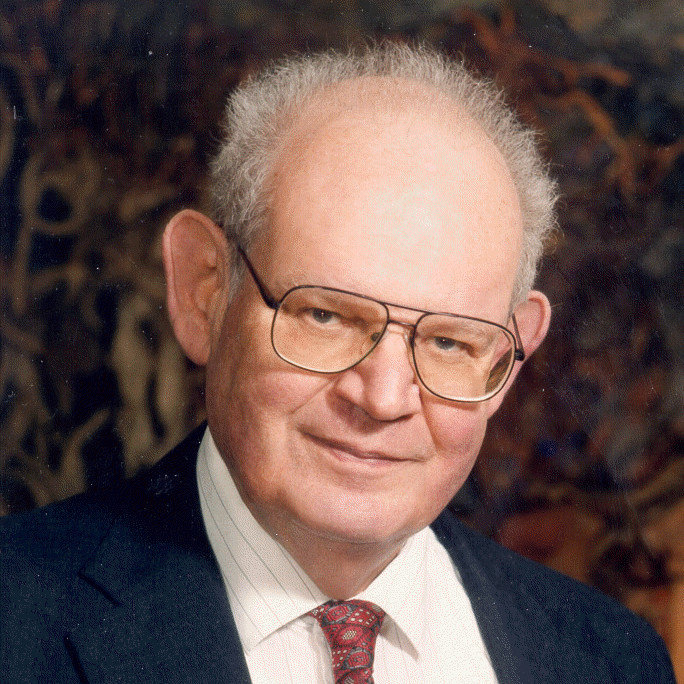
\includegraphics[width=0.5\textwidth]{images/Benoit_B_Mandelbrot.jpeg}}
					% 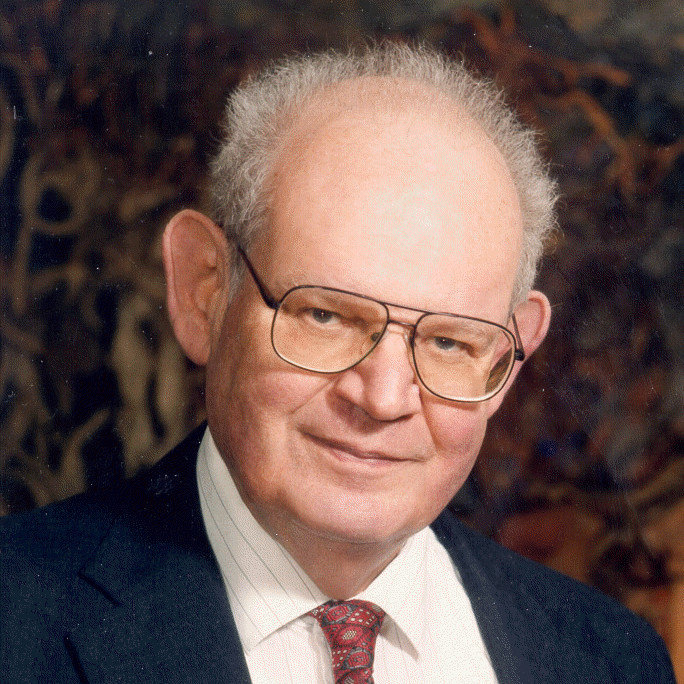
\includegraphics[width=0.5\textwidth]{images/Benoit_B_Mandelbrot.jpeg}
					\caption{Benoit B. Mandelbrot (Nov. 1924 –- Oct. 2010)}
		\end{figure}
		
		\note{
			% https://facts.museum/mandelbrot
			Бенуа Б. Мандельброт. 
			является 
			создателем термина "фрактал" и "фрактальной геометрии"
			
			Термин "Фрактал" появился 1975 г. 
			
			Произошло от
			лат. слова fractus --- фрагментированный, дробный, ломанный.
			
			"Фракталом называется множество, размерность Хаусдорфа-Безиковича которого строго больше его топологической размерности"

			"Все фигуры, которые я исследовал и назвал фракталами, в моем представлении обладали свойством быть нерегулярными, но самоподобными"
			
			Мандельброт Б. "Геометрия природы".
			
					Почему фракталы набрали такую популярность?
				}
	\end{frame}






	\begin{frame}{Эффект Ричардсона. Парадокс береговой линии}
		\begin{figure}
					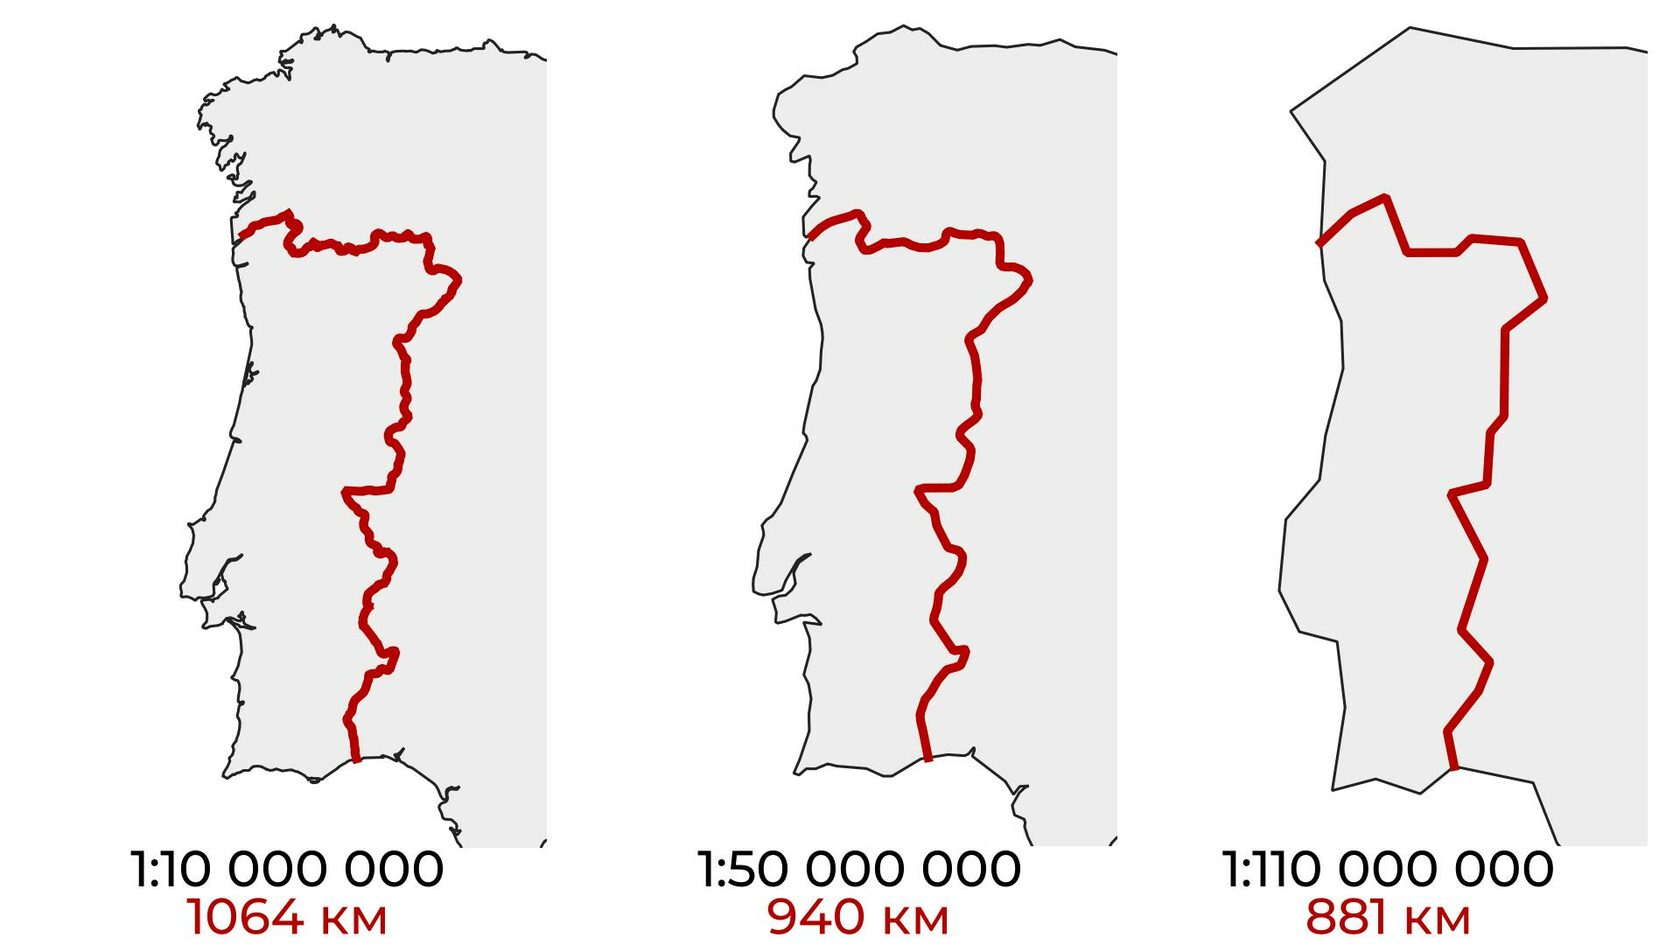
\includegraphics[width=0.9\textwidth]{images/shoreline.jpg}
					\caption{Способы измерения береговой линии}
		\end{figure}
				\note{
					% https://cartetika.ru/tpost/dtulyhzzo1-paradoks-beregovoi-linii
					% https://3dnews.ru/754657
					
					Как посчитать длину кривой между 2 точками?

					\[
						L = R N = R (L/R)^D
						,\]
						где

						$D$ --- фрактальная размерность;
						
						$L$ --- расстояние между двумя точками;
						
						$RN$ --- длина ломанного отрезка;
						
						$R$ --- длина шага с помощью, которого приблизительно пытаемся измерить расстояние.

						Выводы:
						
						Отсюда следует, что при $l \to 0$, $N \to \infty$ 
				}
	\end{frame}



	\begin{frame}{Фрактальная размерность}

		\begin{columns}
			\begin{column}{0.5\textwidth}
				\[
					d = - \lim_{l \to 0} \frac{\ln {N(l)} }{\ln {l}} 
				\]

				Понятие размерности связано с количеством пространственных измерений или степенью многомерности. 
			\end{column}
			\begin{column}{0.5\textwidth}
				\begin{figure}
					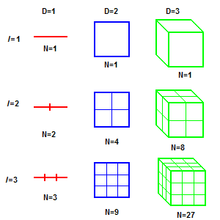
\includegraphics[width=\textwidth]{images/Fractal_dimension_example.png}
					\caption{Определение размерности и масштабирования}
				\end{figure}
			\end{column}
		\end{columns}

		
		
		
		\note{
			% https://en.wikipedia.org/wiki/Fractal_dimension
			% https://stepik.org/lesson/445789/step/8
			
			Рассмотрим следующую цепочку преобразований:
			\[
				\frac{1}{l^d} \approx N(l)
			\]
			\[
				l^d \approx \frac{1}{N(l)}
			\]

			\[
				d 
				= 
				\log_{l}{l^d} \approx \log_{l}{\frac{1}{N(l)}} 
				= 
				\frac{\ln {\frac{1}{N(l)}} }{\ln {l}} 
				= 
				\frac{\ln {N(l)^{-1}} }{\ln {l}} 
				= 
				- \frac{\ln {N(l)} }{\ln {l}} 
			\]

			\[
				d = - \lim_{l \to 0} \frac{\ln {N(l)} }{\ln {l}} 
			\]
			
			Примечание. 
			Если $d$ равняется 1, 2, 3, т.е. $d \in N \cup {0}$, то величина $d$ характеризует евклидову размерность.

			
			Но что будет, если величина $l$ имеет не только целую часть, но и дробную, т.е.
			$d \in  Q$?
			
			% $N \subset Z \subset Q$
		}
	\end{frame}

	\begin{frame}{Способы задания фракталов}
		Структуры, которые представляются фракталами:
		\begin{itemize}
			\item Система реккурентных функций на пространстве;
			\item Стохастический алгоритм;
			\item Итеративная система функций;
			\item L-система (формальная грамматика);
			\item Странный аттрактор (динамические системы);
			\item Конечное правило разделения (рекурсивный способ деления двумерных фигур на меньшие части).
		\end{itemize}

				\note{
					
				}
	\end{frame}

	\begin{frame}{Канторово множество (канторов дисконтинуум, канторова пыль)}

		\begin{columns}
			\begin{column}{0.3\textwidth}
				
				\begin{table}
					% \caption{\label{tab:fractal} Название}
					\begin{center}
						\begin{tabular}{|c|c|c|}
							\hline
							$k$ & $l$ & $N(l)$ \\
							\hline
							0 & $1$ & $1$ \\
							\hline
							1 & $1/3$ & $2$ \\
							\hline
							2 & $1/9$ & $4$ \\
							\hline
							3 & $3^{-3}$ & $2^{3}$ \\
							\hline
							\multicolumn{3}{|c|} {\dots} \\
							\hline
							n & $3^{-n}$ & $2^{n}$ \\
							\hline
						\end{tabular}
					\end{center}
				\end{table}
				
			\end{column}
			\begin{column}{0.7\textwidth}
				\begin{figure}
					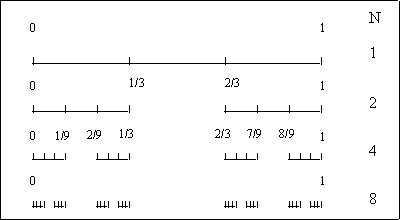
\includegraphics[width=\textwidth]{images/Канторово_множество.png}
					\caption{Схема построения множества Кантора}
		\end{figure}
			\end{column}
		\end{columns}

		\note{
					Множество было описано Георгом Кантором в 1833 году.
					
					Пусть 
					\[
						E_0=[0,1]
						\]
					\[
						E_1=\bigg[ 0,\frac{1}{3}\bigg] \cup \bigg[\frac{1}{3},1\bigg]
						\]
						\[
						E_2
						=
						\bigg[0,\frac{1}{9}\bigg] 
						\cup 
						\bigg[\frac{2}{9},\frac{3}{9}\bigg] 
						\cup 
						\bigg[\frac{6}{9},\frac{7}{9}\bigg] 
						\cup 
						\bigg[\frac{8}{9},1\bigg]
						\]
					\[
						\dots
						\]
				
						Таким образом, множество Кантора строится пересечение отрезков \[P = \bigcap_{n=0}^{\infty} E_n\]
						
						Получается $N=2^n$ сегментов, где $l_i=\frac{1}{3^n}$.
						}
	\end{frame}

	\begin{frame}{Канторово множество}
		\textbf{
		Мера множества после удаления всех отрезков из исходного
		}
		\[
			L = 1 - \frac{1}{3}	 - \frac{2}{9} - \frac{4}{27} - \cdots 
			=
		\]
		\[
			=
			1 - \frac{1}{3} \bigg(	1 + \frac{2}{3} + \frac{4}{9} + \cdots \bigg)
			=
			1 - \frac{1}{3} \cdot 3 = 0
		\]

		\textbf{
		Фрактальная размерность
		}
		\[
			d = - \lim_{n \to \infty} \frac{\ln 2^n }{\ln \frac{1}{3^n}}
			= \log_{3} 2 \approx 0.6309 <1 
		\]

				\note{
					Рассмотрим последовательность
					\[
						S_n = 1 + \frac{2}{3}+ \frac{4}{9} + \cdots
					\]
					
					Эта последовательность является геометрической. Тогда сумму ряда можно вычислить по следующей формуле.
					\[
						S_n = b_1 \cdot \frac{1-q^n}{1-q}
						.
					\]
					Видно, что 
					$b_1 = 1$, $q = \frac{2}{3}$. Тогда сумма ряда равняется

					\[
						S_n= 
						\lim_{n \to \infty} \frac{1- \big(\frac{2}{3}\big)^n }{1- \frac{2}{3}}  
						=
						\frac{1}{\frac{1}{3}} = 3
						.
					\]

				}
	\end{frame}

	\begin{frame}{Снежинка Коха }

		\begin{columns}
			\begin{column}{0.3\textwidth}
				
				\begin{table}
					% \caption{\label{tab:fractal} Название}
					\begin{center}
						\begin{tabular}{|c|c|c|}
							\hline
							$k$ & $l$ & $N(l)$ \\
							\hline
							0 & $1$ & $3$ \\
							\hline
							1 & $1/3$ & $12$ \\
							\hline
							2 & $1/9$ & $48$ \\
							\hline
							\multicolumn{3}{|c|} {\dots} \\
							\hline
							n & $3^{-n}$ & $3 \cdot 4^{n}$ \\
							\hline
						\end{tabular}
					\end{center}
				\end{table}
				
			\end{column}
			\begin{column}{0.7\textwidth}
				\begin{figure}
					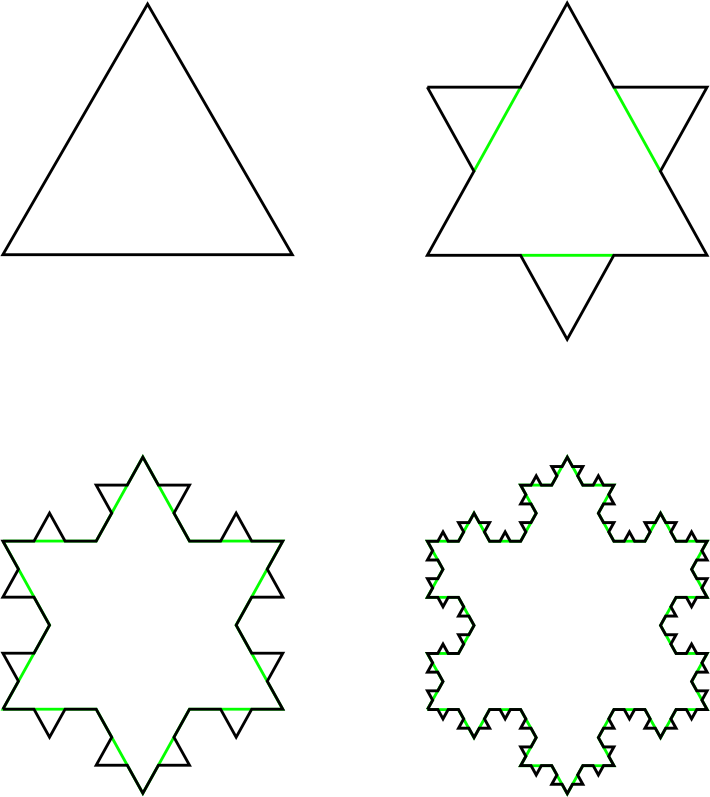
\includegraphics[width=0.6\textwidth]{images/Koch_flake.png}
					\caption{Схема построения снежинки Коха}
		\end{figure}
			\end{column}
		\end{columns}

		\note{
					Множество было описано Кохом (Helge von Koch) в 1904 году.
					
					\textbf{
						Фрактальная размерность
					}
					\[
						d 
						= 
						- \lim_{n \to \infty} \frac{\ln (3\cdot 4^n) }{\ln \frac{1}{3^n}}
						=
						\]
						\[
							=
							\lim_{n \to \infty} \frac{\ln 3 }{\ln {3^n}} +
							\lim_{n \to \infty}  \frac{\ln 4^n }{\ln {3^n}}
							=
							\lim_{n \to \infty} \frac{1}{n} +
							\frac{\ln 4}{\ln {3}}
							=
						\]
						\[
						= 
						\log_{3} 4 \approx 1.26186 > 1
					\]
					}
	\end{frame}

	\begin{frame}{Салфетка Серпинского (треугольник Серпинского)}

		\begin{columns}
			\begin{column}{0.3\textwidth}
				
				\begin{table}
					% \caption{\label{tab:fractal} Название}
					\begin{center}
						\begin{tabular}{|c|c|c|}
							\hline
							$k$ & $l$ & $N(l)$ \\
							\hline
							0 & $1$ & $1$ \\
							\hline
							1 & $1/2$ & $3$ \\
							\hline
							2 & $1/4$ & $9$ \\
							\hline
							\multicolumn{3}{|c|} {\dots} \\
							\hline
							n & $2^{-n}$ & $3^{n}$ \\
							\hline
						\end{tabular}
					\end{center}
				\end{table}
				
			\end{column}
			\begin{column}{0.7\textwidth}
				\begin{figure}
					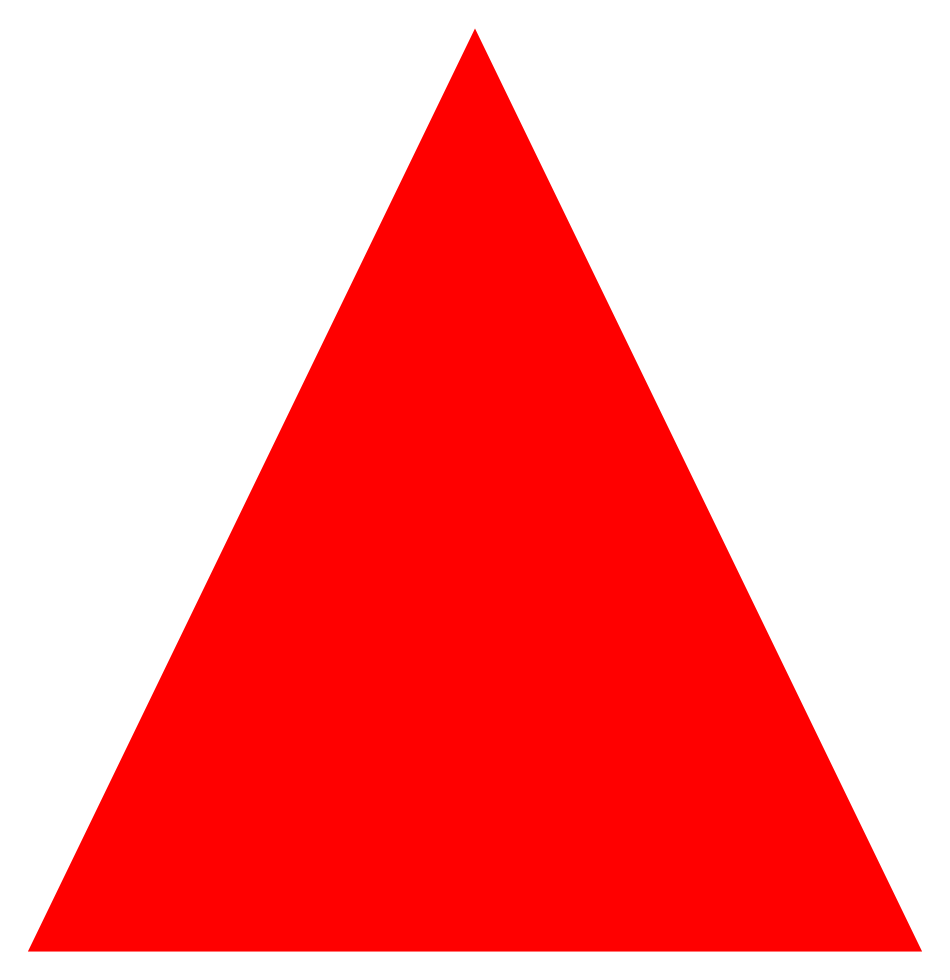
\includegraphics[width=0.35\textwidth]{images/1.png}
					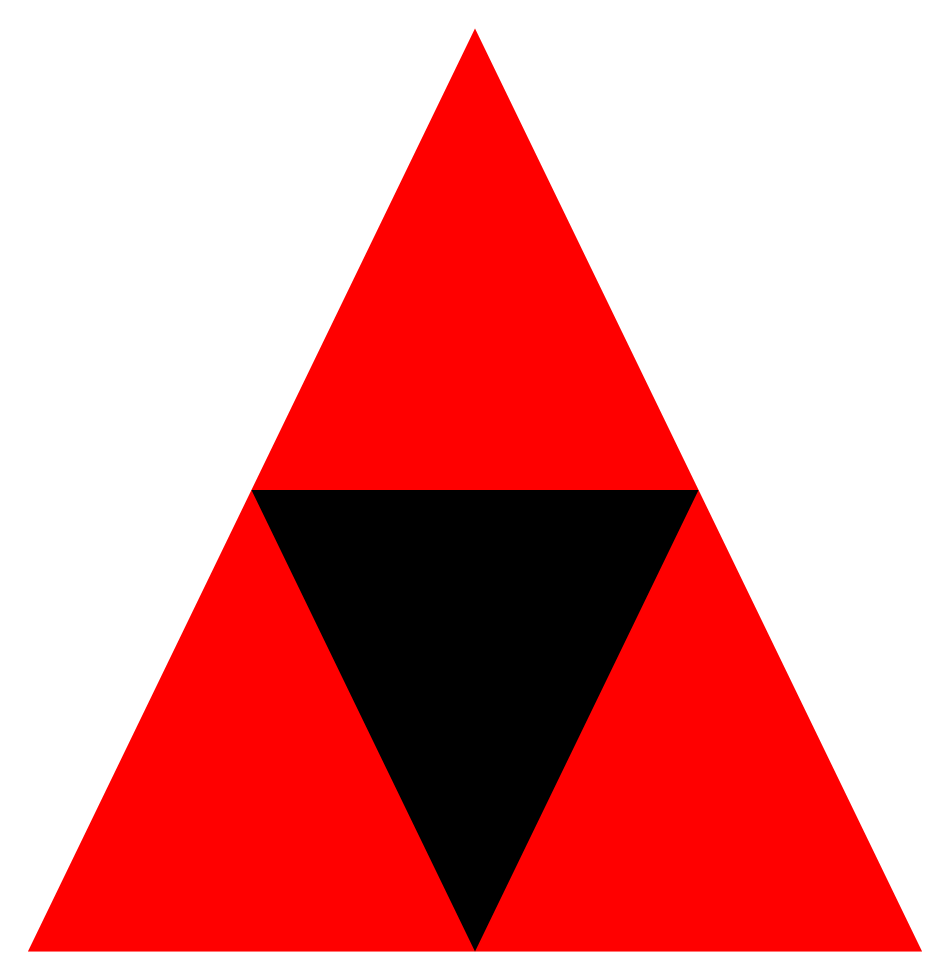
\includegraphics[width=0.35\textwidth]{images/2.png}
					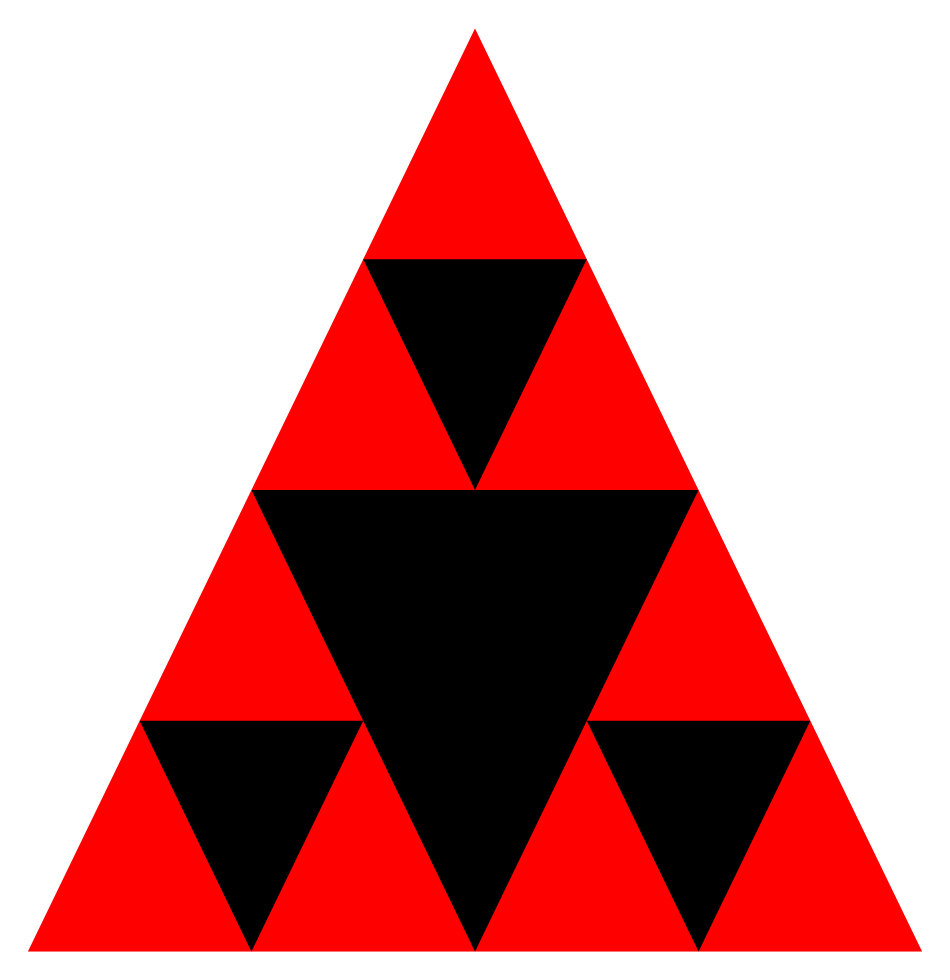
\includegraphics[width=0.35\textwidth]{images/3.png}
					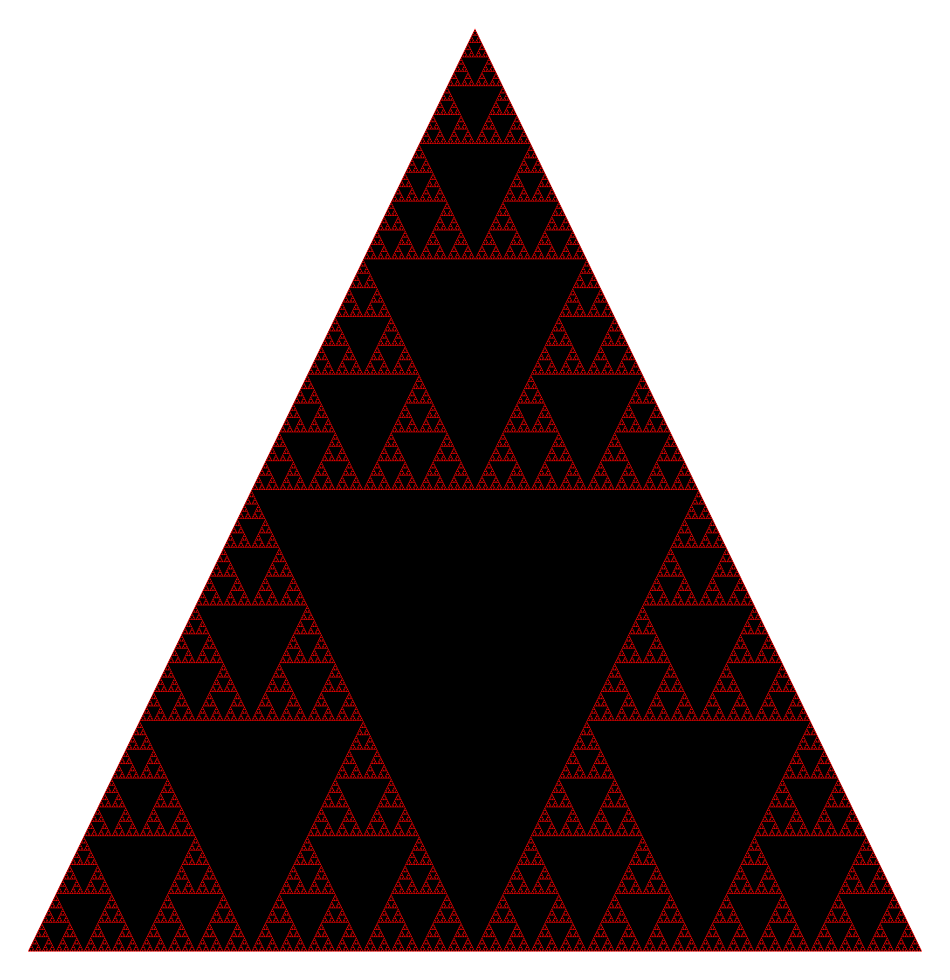
\includegraphics[width=0.35\textwidth]{images/10.png}
					\caption{Схема построения салфетки Серпинского}
		\end{figure}
			\end{column}
		\end{columns}

		\note{
					Множество было описано Серпинским в 1916 году.
					
					\textbf{
					Площадь объекта
					}
					\[
					S =	1 - \frac{1}{4}(1 + \frac{3}{4} + \cdots) = 1 - \frac{1}{4}\cdot 4 = 0
					\]

					\textbf{
						Фрактальная размерность
					}
					\[
						d 
						= 
						- \lim_{n \to \infty} \frac{\ln 3^n }{\ln \frac{1}{2^n}}
						=
						\frac{\ln 3 }{\ln 2}
						=
						\]
						\[
						= 
						\log_{2} 3 \approx 1.58496250072  > 1
					\]

					}
	\end{frame}

	\begin{frame}{Алгебраические фракталы}

		Пусть задана рекуррентная функция в комплексной плоскости
		$z_{n+1} = f(z_n),$ где $z_n \in Z$.
		% т.е. дано отображение вида 		$f : С \to С$.
		
		Установим некоторое начальное значение $z_0$ и рассмотрим последовательность вида $\{z_0, z_1, z_2, \dots , z_n \}$.

		В зависимости от начальных данных, т.е. от $z_0$, последовательность ведет себя по-разному. При $n \to \infty$ возможны следующие значения функции:
		\begin{enumerate}
			\item $z_n \to \infty$, т.е. $\lim_{n \to \infty} f(z_n) = \infty$;
			\item $z_n = A$, т.е. $\lim_{n \to \infty} f(z_n) = A$;
			\item $z_n = z_{n+ \tau}$, где  $\tau$ --- период, т.е. $z_n$ циклически принимает некоторый ряд значений.
		\end{enumerate}

				\note{

				Операции над комплексными числами.

				Сложение комплексных чисел $z_1= a+bi$ и $z_2 =c+di$:
				\[
					\left(a+bi\right) + \left(c+di\right) = \left(a+c\right) + \left(b+d\right)i,
				\]

				Произведение комплексных чисел $a+bi$ и $c+di$:
				\[
				\left(a+bi\right) \cdot \left(c+di\right) = ac+bci+adi+bdi^2 
				=
				\] 
				\[
				=
				\left(ac+bdi^2\right) +\left(bc+ad\right)i=\left(ac-bd\right)+\left(bc+ad\right)i.
				\]
				}
	\end{frame}

	\begin{frame}{Алгебраические фракталы}

		% Написать строгую формулировку
		Рассмотрим производную такой функции:
		\[
			f'(z) = \lim_{\Delta z \to 0} \frac{f(z + \Delta z)-f(z)}{\Delta z}
			.
		\]
		Выполним ряд преобразований и в результате получим:

		\[
			f(z + \Delta z) \approx f(z) + \Delta z f'(z) 
			.
		\]

		Отсюда следует, что расстояние между точками можно задать через производную.
		Предположим, что существует неподвижная точка $\hat{z}$ --- корень уравнения функции, тогда, если
\begin{enumerate}
\item $|f' \hat{z} | < 1$, то $\hat{z}$ --- притягивающая точка;
\item $|f'\hat{z}| > 1$, то $\hat{z}$ --- отталкивающая точка;
\item $|f'\hat{z}| = 1$, то $\hat{z}$ --- нейтральная точка.
\end{enumerate}
		

				\note{


					Должно выполняться условие Коши-Римана.
					\[
						\frac{\partial f}{\partial a} + i \frac{\partial f}{\partial b} = 0,
					\]
				}
	\end{frame}


	\begin{frame}{Множество Мандельброта. Множество Жюлиа}
		
		\begin{figure}
			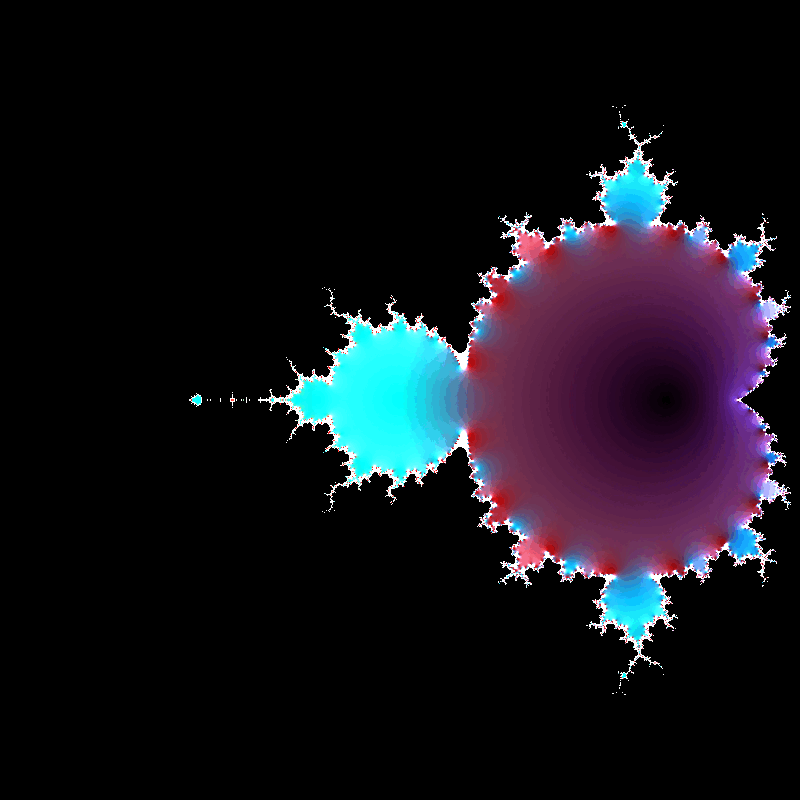
\includegraphics[width=0.45\textwidth]{images/mandelbrot_set.png}
			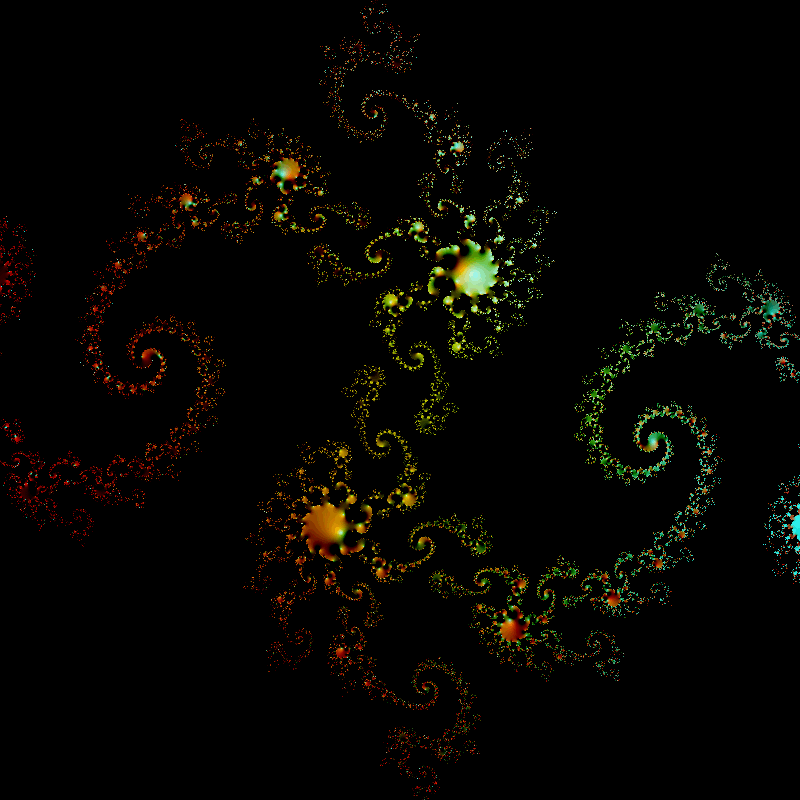
\includegraphics[width=0.45\textwidth]{images/julia_set.png}
			\caption{Множество Мандельброта (слева) и Жюлиа (справа)}
		\end{figure}
		
		\note{

		Определение и название принадлежат французскому математику Адриену Дуади.

					\[
						z_{n+1} = z_n^2+c
						, 
						\]
					где $c$ --- некоторая константа.			
					
					Характеристики множества Мандельброта:
					\begin{itemize}
						\item Кардиоида (периода);
						\item Иголоподобные антенны.
					\end{itemize}
			
				}
	\end{frame}


	\begin{frame}{L-systems (L-системы)}
		L-системы --- тип формальной грамматики.

		L-система задается $G = (V, \omega, P )$, где
	
		\begin{itemize}
			\item $V$(алфавит) --- множество символов, содержащих как элементы, которые могут быть заменены (переменные), так и элементы, которые не могут быть заменены (”константы”или ”терминальные символы”);
			\item $\omega$ --- (старт) строка символов из $V$, определяющая начальное состояние системы;
			\item $P$ --- множество правил, определяющих, каким образом переменные могут быть заменены комбинациями констант и других переменных. Порождающее правило состоит из двух строк, прототип и преемник.
		\end{itemize}

	\note{
		Такой способ построения предложил в 1968 Аристид Линденмайер, венгерский биолог и ботаник из Утрехтского университета. Он использовал L-системы для описания поведения клеток растений и моделирования процесса развития растения.
	}
	\end{frame}

	\begin{frame}{L-systems (L-системы)}
		Пример. Множество Кантора
	
		\begin{itemize}
			\item переменные: $A, B$
			\item константы: нет
			\item старт: $A$
			\item правила: $(A \to ABA), (B \to BBB)$
		\end{itemize}

		Пусть $A$ означает «рисуем отрезок», а $B$ означает «движемся».
		
	\note{
		Такая грамматика порождает знаменитое канторово фрактальное множество на вещественной оси R.

		Шаг 0.

		$A$

		Шаг 1.

		$ABA$

		Шаг 2.

		$ABABBBABA$

	}
	\end{frame}

	\begin{frame}{L-systems (L-системы)}
		Пример. Треугольник Серпинского
	
		\begin{itemize}
			\item переменные: $F, G$
			\item константы: $+, -$
			\item старт: $F-G-G$
			\item правила: $(F \to F-G+F+G-F), (G \to GG)$
			\item угол: 120\textdegree
		\end{itemize}

		Здесь $F$ и $G$ означают «рисуем отрезок», 
		$+$ означает «повернуть вправо на угол», 
		а $-$ означает «повернуть влево на угол».
		
	\note{
		Такая грамматика порождает знаменитое канторово фрактальное множество на вещественной оси R.

		Шаг 0.

		$F-G-G$

		Шаг 1.

		$F-G+F+G-F-GG-GG$

		Шаг 2.

		$F-G+F+G-F-GG+F-G+F+G-F+GG-F-G+F+G-F-GGGG-GGGG$

	}
	\end{frame}


	\begin{frame}{Стохастические фракталы}
		\begin{figure}
					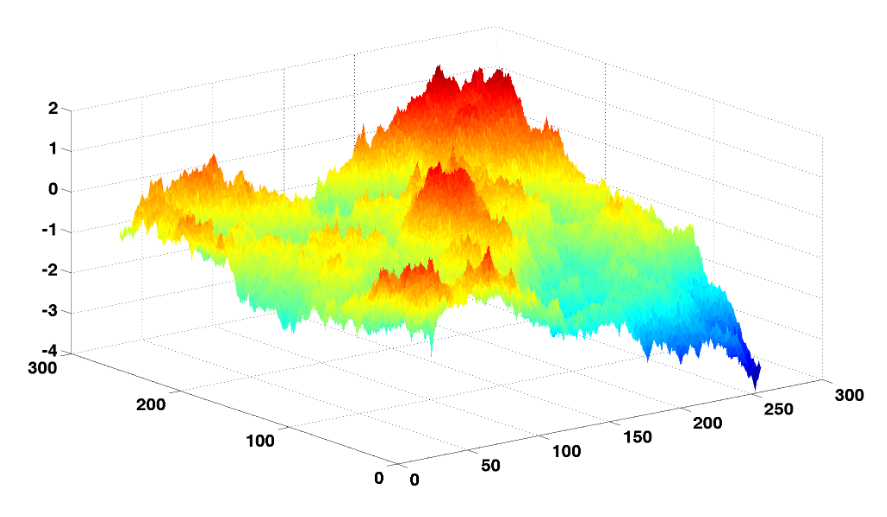
\includegraphics[width=0.9\textwidth]{images/stochastic-fractal-1.png}
					\caption{Генерация обобщенного броуновского рельефа}
		\end{figure}
				\note{
					Стохастические фракталы являются известным классом фракталов. Они
нашли широкое применение в области создания природных несимметричных объектов,
таких как ландшафты, деревья и облака. 


						Способы построения
						% https://habr.com/ru/articles/111538/
						\begin{itemize}
							\item алгоритм случайного блуждания;
							\item алгоритм Diamond-square.
						\end{itemize}
				}
	\end{frame}

	\begin{frame}{Построение салфетки Серпинского с помощью метода случайных итераций}
		\begin{figure}
					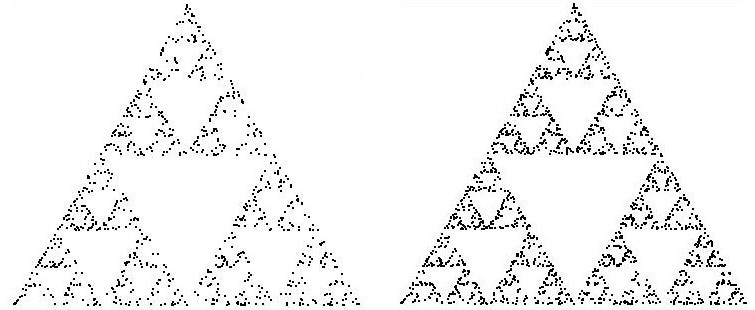
\includegraphics[width=0.6\textwidth]{images/sierpinski-3panel.jpg}
					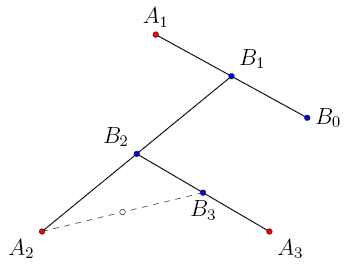
\includegraphics[width=0.3\textwidth]{images/sierpinski-algorithm.png}
					\caption{Игра "Хаос" (слева) и алгоритм построения (справа)}
		\end{figure}
			\note{
				Получается в результате случайного блуждания точки на плоскости. Этот способ называется «игрой Хаос». С его помощью можно построить и некоторые другие фракталы.

				Суть «игры» такова. 
				
				На плоскости зафиксирован правильный треугольник A1A2A3. Отмечают любую начальную точку B0. Затем случайным образом выбирают одну из трех вершин треугольника и отмечают точку B1 — середину отрезка с концами в этой вершине и в B0 (на рисунке справа случайно выбралась вершина A1). 
				
				Затем повторяют с точкой B1, чтобы получить B2. Потом получают точки B3, B4, и т. д. 
				
				Важно, чтобы точка «прыгала» случайным образом, то есть чтобы каждый раз вершина треугольника выбиралась случайно, независимо от того, что было выбрано в предыдущие шаги. Удивительно, что если отмечать точки из последовательности Bi, то вскоре начнет проступать треугольник Серпинского.
			}
	\end{frame}


	\begin{frame}{Алгоритм Diamond-square}
		\begin{figure}
					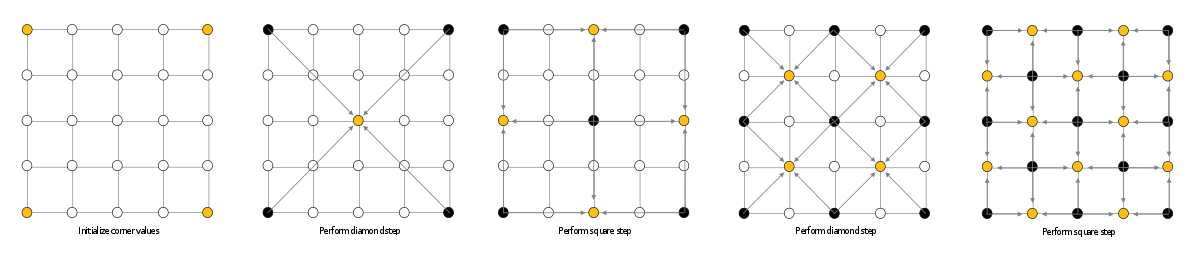
\includegraphics[width=\textwidth]{images/Diamond_Square.png}
					\caption{Схема алгоритма Diamond-square}
		\end{figure}
				\note{
					Описание алгоритма было впервые представлено в 1982 г (by Fournier, Fussell and Carpenter at SIGGRAPH).

					Алгоритм Diamond-square

\begin{enumerate}
	\item Инициализация угловых точек. Присваивание им значений высот (например, выбором случайных чисел).
	\item Шаг diamond. Нахождение срединной точки, присваивание ей значения, на основе среднего от угловых, плюс случайное число.
	\item Шаг square. Нахождение срединных точек для ромбов отмеченных черными точками (на этом шаге, по одной точке каждого ромба выходят за пределы массива). Плюс случайное число. 
\end{enumerate}
				}
	\end{frame}

	\begin{frame}{Стохастические фракталы}
		\begin{figure}
					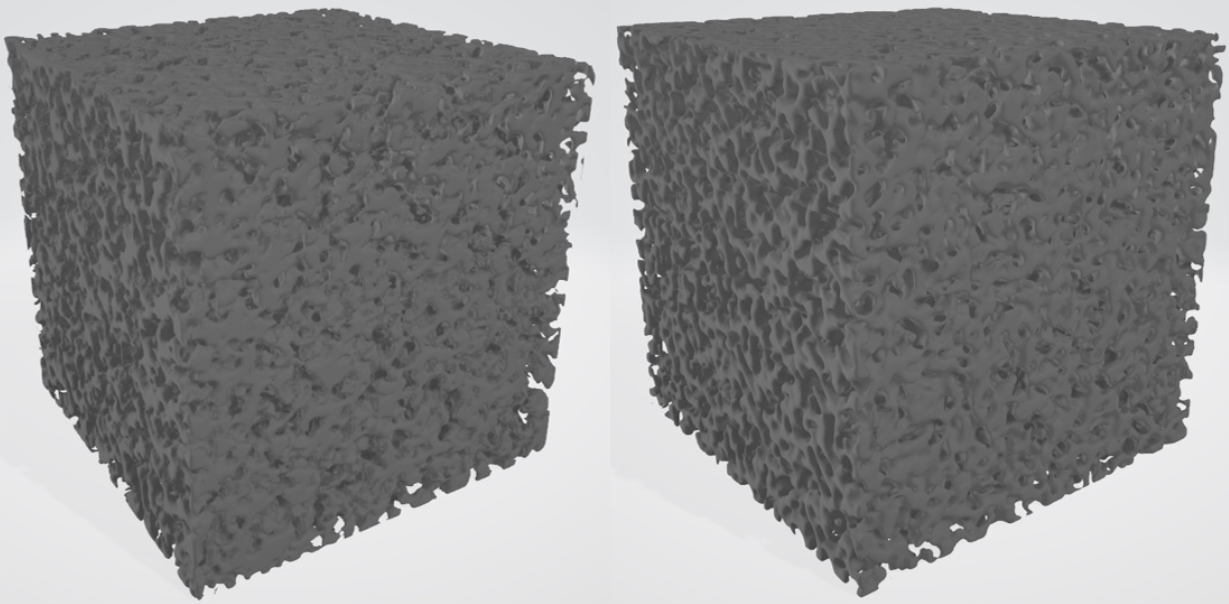
\includegraphics[width=\textwidth]{images/stochastic-fractal-2.png}
					\caption{Построение пористой среды с помощью шума Перлина (слева) газового фрактала (справа)}
		\end{figure}
				\note{
					В качестве цифровых моделей пористых сред были использованы фрактальные пористые структуры, созданные на основе стохастических фракталов: шум Перлина и газовое облако на основе алгоритма Octahedron and Cube.
				}
	\end{frame}


\end{document}

	\begin{frame}{Стохастические фракталы}
		\begin{figure}
					% 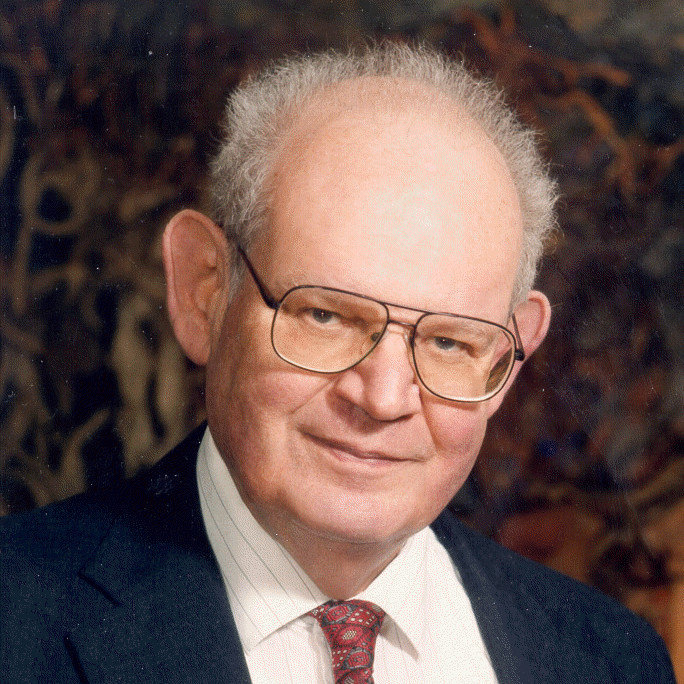
\includegraphics[width=\textwidth]{images/Benoit_B_Mandelbrot.jpeg}
					\caption{Фрактал обыкновенный}
		\end{figure}
				\note{
					Пояснение
				}
	\end{frame}
\end{document}


\begin{frame}{История фракталов}
	\begin{figure}
				% 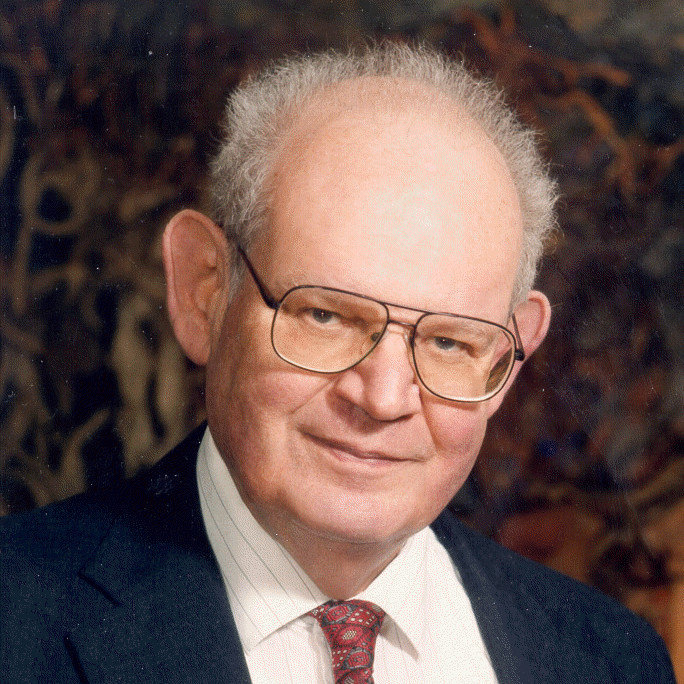
\includegraphics[width=\textwidth]{images/Benoit_B_Mandelbrot.jpeg}
				\caption{Фрактал обыкновенный}
	\end{figure}
			\note{
				Примеры фракталов:
				1. Леонардо да Винчи ствол
				2. Фрактальные структуры Биологический закон Мюллера и Гекеля
				3. Фрактальное сжатие игра
			}
\end{frame}